\kommentar{Leitungen}

\begin{karte}{Was ist eine Leitung?}
	Für uns ist eine Leitung eine Wellenführung.\\
	\divTwo{
		\textbf{Ungeführte Welle:}
		%Autor: Simon Walker
%Version: 1.0
%Datum: 24.04.2020
%Lizenz: CC BY-NC-SA

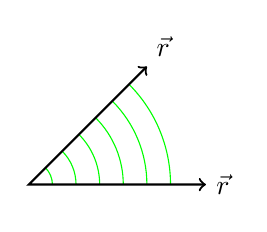
\begin{tikzpicture}[smooth, xscale=0.5, yscale=0.5]
	%\HelpCords{0}{0}{5}{4}
	
	\foreach \x in {0.6, 1.2, ...,4}{
		\draw[green] (\x, 0) arc (0:45:\x);	
	}
	
	\draw[<->, thick] (3, 3) -- (0, 0) -- (4.5, 0) node[right] {$\vec{r}$};
	\node[above right] at (3, 3) {$\vec{r}$};
\end{tikzpicture}
\\
		\scalebox{.7}{%Autor: Simon Walker
%Version: 1.0
%Datum: 24.04.2020
%Lizenz: CC BY-NC-SA

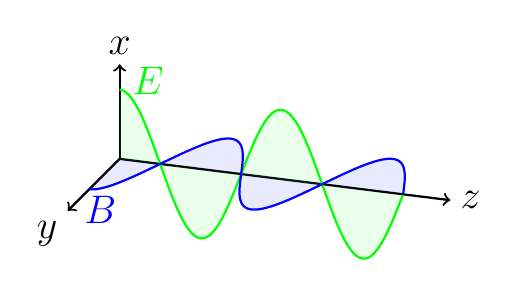
\begin{tikzpicture}[x={(0,0.8cm)}, y={(-0.55cm,-0.55cm)}, z={(1.2cm, -0.15cm)}]
		
	\def\cycles{1.75} %Anz Schwingungen
	\def\lenght{3}%länge in z richtung
	
	
	\draw [->, thick] (0,0,0)  -- (1.5,0,0) node[above] {\Large$x$};
	\draw [->, thick] (0,0,0) -- (0,1.2,0) node[below left] {\Large$y$};
	\draw [->, thick] (0,0,0) -- (0,0,\lenght+0.5) node[right] {\Large$z$};
	
	\draw[thick, green] %E-Feld Plot
	plot[domain=0:\lenght, samples=200] 
	({1.1*cos(deg(2*\cycles*pi*\x/\lenght))}, 0, \x);
	
	\draw[thick, blue] %M-Feld Plot
	plot[domain=0:\lenght, samples=200] 
	(0, {0.7*cos(deg(2*\cycles*pi*\x/\lenght))}, \x);
	
	\fill[opacity=.1,green!80] %E-Feld füllung
	(0,0,0) --
	plot[domain=0:\lenght, samples=200] 
	({1.1*cos(deg(2*\cycles*pi*\x/\lenght))}, 0, \x)  --
	(0,0,0);
	
	\fill[opacity=.1,blue!80] %M-Feld füllung
	(0,0,0) --
	plot[domain=0:\lenght, samples=200] 
	(0, {0.7*cos(deg(2*\cycles*pi*\x/\lenght))}, \x)  --
	(0,0,0);
	
	\node[green] at (1.3,0,0.3) {\Large$E$}; %Beschriftungen
	\node[blue] at (0,1.1,0.3) {\Large$B$};
	
\end{tikzpicture}
}
		\centering
		$\vec{k} \cdot \vec{r}$
		
	}{
		\textbf{Geführte Welle:}\\[5pt]
		%Autor: Simon Walker
%Version: 1.0
%Datum: 24.04.2020
%Lizenz: CC BY-NC-SA

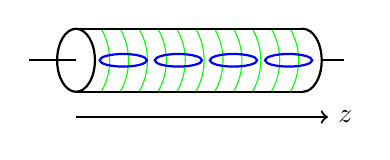
\begin{tikzpicture}[smooth, xscale=0.4, yscale=0.4]
%	\HelpCords{0}{-1}{9}{1}

	\draw[thick] (-0.5, 0) -- (1, 0);
	\draw[thick] (8, 0) -- (9.5, 0);
	
	\draw[thick] (1, 0) ellipse circle [x radius=0.6, y radius=1];
	
	\draw[thick, fill=white] (8.2, 0) ellipse circle [x radius=0.6, y radius=1];
	\fill[white] (7,-1) rectangle (8.2,1);
	
	\foreach \x in {1.8, 2.4, ...,8}{
		\draw[green] (\x, -1) arc (-30:30:2);	
	}
	
	\draw[thick] (1, 1) -- (8.2, 1);
	\draw[thick] (1, -1) -- (8.2, -1);
	
	\foreach \x in {2.5, 4.25, ..., 8}{
		\draw[thick, blue] (\x, 0) ellipse circle [x radius=0.75, y radius=0.2];
	}

	\draw[thick, ->] (1, -1.8) -- (9, -1.8) node[right] {$z$};
\end{tikzpicture}

		\begin{center}
			$k\cdot z = \beta z \quad \Rightarrow \quad k=\beta$
		\end{center}
		Im Beispiel ist ein Koaxialleiter zu sehen. Das $B$-Feld ist Ortogonal zum $E$-Feld. Die gesamte Anordnung ist Symetrisch.
	}
\end{karte}

\begin{karte}{Wie Sieht das Schema des Leitungsmodells aus?}
	Das Leitungsmodell bezieht sich auf einen kurzen Leitungsausschnitt. Dadurch erhalten wir längenunabhängige Kenngrössen die sogenanten Leitungsbeläge.\\
	\scalebox{.49}{%Autor: Simon Walker
%Version: 1.0
%Datum: 04.06.2020
%Lizenz: CC BY-NC-SA

\begin{circuitikz}
	%\HelpCords{0}{0}{8}{-4}
	
	
	\draw
	%Knoten
	(0, 0) coordinate (n1)
	
	($(n1)+(0.1,0)$) coordinate(n11)
	
	(1.5, 0) coordinate (n2)
	(3.5, 0) coordinate (n3)
	(5.5, 0) coordinate (n4)
	
	($(n4)+(0,-0.1)$) coordinate(n41)
	
	(8, 0) coordinate (n5)
	
	($(n5)+(-0.1,0)$) coordinate(n51)
	
	
	($(n4)+(0, -1)$) coordinate (n6)
	($(n6)+(0, +0.1)$) coordinate (n60)
	($(n6)+(-0.8, 0)$) coordinate (n61)
	($(n6)+(0.8, 0)$) coordinate (n62)
	
	($(n6)+(0, -2)$) coordinate (n7)
	($(n61)+(0, -2)$) coordinate (n71)
	($(n62)+(0, -2)$) coordinate (n72)
		
	($(n7)+(0, -0.5)$) coordinate (n9)
	
	(8, -3.5) coordinate (n8)
	(0, -3.5) coordinate (n10)
	
	
	
	%Nur zu Hilfszwecken
%	(n1) node[above] {$n1$}
%	(n2) node[above] {$n2$}
%	(n3) node[above] {$n3$}
%	(n4) node[above] {$n4$}
%	(n5) node[above] {$n5$}
%	(n6) node[above] {$n6$}
%	(n7) node[above] {$n7$}
%	(n8) node[above] {$n8$}
%	(n9) node[above] {$n9$}
%	(n10) node[above] {$n10$}
%	
%	(n11) node[below] {$n11$}
%	(n41) node[below] {$n41$}
%	(n51) node[below] {$n51$}
%	(n60) node[below] {$n60$}
%	(n61) node[above] {$n61$}
%	(n62) node[above] {$n62$}
%	(n71) node[above] {$n71$}
%	(n72) node[above] {$n72$}
	
	(n1) to [short,o-] (n11)
	(n11) to[short,color=red,i=${\color{red} i(z,t)}$] (n2)
	(n2) to[R=$R'dz$] (n3)
	(n3) to [american inductor=$L'dz$] (n4)
	(n4) to[short, color=red, i=${\color{red} i(z+dz,t)}$] (n51)
	(n51) to[short,-o] (n5)
	
	(n4) to[short, *-] (n41)
	(n41) to[short, color=red, i=${\color{red} \Delta i(z,t)}$] (n60)
	(n60) to[short, -*] (n6)
	(n6) to[short] (n61)
	(n6) to[short] (n62)
	(n61) to[R,l_=$G'dz$] (n71)
	(n62) to[C=$C'dz$] (n72)	
	(n7) to[short] (n71)
	(n7) to[short] (n72)
	(n7) to[short, *-*] (n9)
	
	(n10) to[short, o-o] (n8)
	;
	
	\draw[|<->|] ($(n10)+(0,-0.7)$) --
	node[above] {$dz$}
	($(n8)+(0,-0.7)$);
	
	\draw[blue,->] (0.3, 0.6) to[out=10,in=170] (7.3, 0.6);
	\node[above, blue] at (3.75, 0.9) {$\Delta u(z)$};
	
	
	\draw[blue,->] ($(n1)+(0, -0.3)$) --
	node[left, blue] {$u(z,t)$}
	($(n10)+(0, +0.3)$);
	
	\draw[blue,->] ($(n5)+(0, -0.3)$) --
	node[right, blue] {$u(z+dz,t)$}
	($(n8)+(0, +0.3)$);
	
\end{circuitikz}}\\[5pt]
	\tiny
	\renewcommand\arraystretch{1.7}
	\begin{tabular}{cl}
		$R'=\frac{dR}{dz}$ & Widerstandsbelag in $\Omega/m$\\
		$L'=\frac{dL}{dz}$ & Induktivitätsbelag in $H/m$\\
		$G'=\frac{dG}{dz}$ & Isolationsbelag in $S/m$\\
		$C'=\frac{dC}{dz}$ & Kapazitätsbelag in $F/m$\\
	\end{tabular}
	\normalsize
\end{karte}

\begin{karte}{Was ist eine TEM-Welle?}
	TEM steht für transversalelektomagnetisch. Eine TEM-Welle hat nur Komponenten, welche senkrecht zur Ausbreitungsrichtung sind. Im Bild ist $z$ die Ausbreitungsrichtung der Welle und steht senkrecht zu $\vec{E}$ und $\vec{H}$. \\[10pt]
	%Autor: Simon Walker
%Version: 1.0
%Datum: 28.04.2020
%Lizenz: CC BY-NC-SA

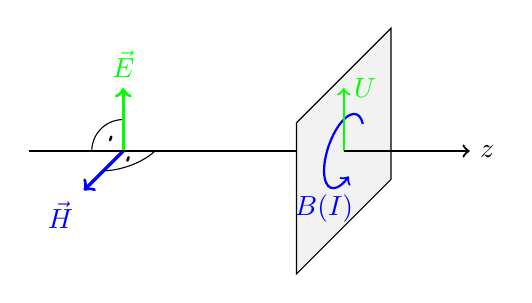
\begin{tikzpicture}[x={(0, 0.8cm)}, y={(-0.5cm,-0.5cm)}, z={(0.8cm, 0)}]

\def\l{7} %länge der z-Achse
\def\s{1.2} %Quadratgrösse (eine Seite ist s*2)
\def\p{5} %Positoon des Quadrates

\draw[domain=90:180,smooth,variable=\x] plot ({sin(\x)*0.5},{0}, {1.5+cos(\x)*0.5});
\draw[domain=0:90,smooth,variable=\x] plot ({0},{sin(\x)*0.5}, {1.5+cos(\x)*0.5});
\draw[fill=black] (0.2, 0, 1.3) circle[radius=0.03];
\draw[fill=black] (0, 0.2, 1.7) circle[radius=0.03];
\draw[very thick, green, ->] (0, 0, 1.5) -- (1, 0, 1.5) node[above, green] {$\vec{E}$};
\draw[very thick, blue, ->] (0, 0, 1.5) -- (0, 1, 1.5) node[below left, blue] {$\vec{H}$};

\draw[thick] (0, 0, 0) -- (0, 0, \p); %Beginn der Z-Achse

\draw[fill=gray!10] (-\s, -\s, \p) -- (-\s, \s, \p) -- (\s, \s, \p) -- (\s, -\s, \p) -- cycle;
\draw[->,domain=-75:195,smooth,variable=\x, blue, thick] plot ({cos(\x)*0.5},{sin(\x)*0.5}, {\p});
\node[blue] at (-0.6, 0.5, \p) {$B(I)$};
\draw[->, green, thick] (0, 0, \p) -- (1, 0, \p) node[right, green] {$U$};
\draw[thick, ->] (0, 0, \p) -- (0, 0, \l) node[right] {$z$}; %Ende der Z-Achse

\end{tikzpicture}

\end{karte}

\begin{karte}{Was bedeutet der Begriff Wellenimpedanz?}
	Die Wellenimpedanz ist das Verhältnis zwischen Spannung und Strom der Welle. Achtung: Dies ist nicht gleich der gemessenen Spannung und Strom an einem gewissen Punkt $z$ in der Leitung!\\[5pt]
	%Autor: Simon Walker
%Version: 1.0
%Datum: 30.04.2020
%Lizenz: CC BY-NC-SA

\begin{tikzpicture}[smooth, xscale=0.6, yscale=0.6]
%	\HelpCords{0}{-1}{9}{1}

	\draw[thick] (-1, 0) -- (1, 0);
	\draw[thick] (8, 0) -- (10.5, 0);
	
	\draw[thick] (1, 0) ellipse circle [x radius=0.6, y radius=1];
	
	\draw[thick, fill=white] (8.2, 0) ellipse circle [x radius=0.6, y radius=1];
	\fill[white] (7,-1) rectangle (8.2,1);
	
	
	\draw[thick] (1, 1) -- (8.2, 1);
	\draw[thick] (1, -1) -- (8.2, -1);
	
	%Pfeile
	\draw [->, blue] (2, 0) -- ++(0.3,0) 
	arc [radius=0.2, start angle=180, end angle = 0] 
	arc [radius=0.2, start angle=-180, end angle = 0]
	arc [radius=0.2, start angle=180, end angle = 0] -- ++(0.3,0);
	\node [blue] at (3, 0.6) {$U_+$};
	\node [blue] at (3, -0.6) {$I_+$};
	
	\draw [->, blue] (8, 0) -- ++(-0.3,0) 
	arc [radius=0.2, start angle=0, end angle = 180] 
	arc [radius=0.2, start angle=0, end angle = -180]
	arc [radius=0.2, start angle=0, end angle = 180] -- ++(-0.3,0);
	\node [blue] at (7, 0.6) {$U_-$};
	\node [blue] at (7, -0.6) {$I_-$};

	\draw[thick, ->] (1, 1.7) -- (9, 1.7) node[right] {$z$};
	
	\draw[very thick, ->] (2, -1.3) -- ++(0, -1.2) -- ++(1.2, 0) node [right]
	{$Z_0 = \color{blue} \dfrac{U_+}{I_+} \color{black} = 
	\color{blue} \dfrac{U_-}{I_-} \color{red} \ne \dfrac{U(z)}{I(z)}$}; 
	\node[right] at (3.2, {-2.5-1.3}) 
	{$\color{white} Z_0 \color{black} = \sqrt{\frac{R'+j \omega L'}{G' +j \omega C'}}= Z(\omega) \text{\tiny{\quad gemäss Leitungsmodel}}$} ;
	
\end{tikzpicture}
 
\end{karte}

\begin{karte}{Was bezeichnet man als Ausbreitungsgeschwindigkeit?}
	Für uns ist meistens mit der Ausbreitungsgeschwindigkeit die Phasengeschwindigkeit gemeint.
	\begin{equation*}
		v = \frac{dz}{dt} = v_{ph} 
	\end{equation*}
	Am einfachsten wird geschaut wie sich der Peak der Welle fortbewegt.
	\vspace{-10pt}
	\begin{figure}[h]
		\centering
		%Autor: Simon Walker
%Version: 1.0
%Datum: 30.04.2020
%Lizenz: CC BY-NC-SA

\begin{tikzpicture}[xscale=0.7, yscale=0.7]
	%\HelpCords{0}{-1}{9}{1}
	
	\def\l{8} %Länge der Schwingungen
	\def\o{0.9} %Offset (Positiv bedeutet Rot links von blau)
	\def\f{0.3} %Frequenz der Schwingunen
	
	\tikzmath{
		\p1 = 450/(360*\f); %Peek1
		\p2 = \p1 - \o; %Peek2
		\pl = (\p1+\p2)/2;
	}
	
	\draw[blue] plot[domain=0:\l, samples=200] 
	(\x, {sin(360*\f*\x});
	\draw[red] plot[domain=0+\o:\l+\o, samples=200] 
	(\x-\o, {sin(360*\f*\x)});
	
	%\draw[green, *<-*] (\p2, 1) -- (\p1, 1);
	\draw [thick] (\p1, 1) -- (\p1, 1.5);
	\draw [thick](\p2, 1) -- (\p2, 1.5);
	\draw [->, thick] (\p1, 1.25) -- (\p2, 1.25);
	\node[above] at (\pl, 1.25) {$dz$};
	
	\draw[fill=green, green] (\p1, 1) circle [radius=0.08];
	\draw[fill=green, green] (\p2, 1) circle [radius=0.08];
	
\end{tikzpicture}

	\end{figure}
\end{karte}

\begin{karte}{Was ist die Ausbreitungskonstante?}
	Die Ausbreitungskonstante $\gamma$ ist eine komplexe Grösse und hat die Einheit $Np/m + jrad/m$. $Np/m$ ist (Neper/Meter).\\[7pt]
	\begin{minipage}[c]{0.38\textwidth}
		\begin{equation*}
		\gamma = \alpha + j \beta
		\end{equation*}
	\end{minipage}
	\begin{minipage}[t]{0.68\textwidth}
		\begin{tabular}{ccl}
			$\gamma$ & => & Ausbreitungskonstante\\
			$\alpha$ & => & Dämpfungskonstante\\
			$\beta$  & => & Phasenkonstante
		\end{tabular}
	\end{minipage}\\[7pt]
	
	Eine Welle kann mittels der Ausbreitungskonstante definiert werden:
	\begin{equation*}
		U_+ e^{-\gamma z}
	\end{equation*}
	Wobei $U_+ e^{-\gamma z}$ eine Welle in die Positive $z$ Richtung ist mit der komplexen Amplitude $U_+=|U_+| e^{j \varphi_+}$
\end{karte}

\begin{karte}{Wie entstehen durch Leitungen Verzerrungen und wie können diese verhindert werden?}
	Eine Möglichkeit ist die \textbf{Dispersion}. Dies ist dann der Fall wenn $\beta(\omega)$, $\gamma(\omega)$, $Z(\omega)$, $v(\omega)$ Frequenzabhänig sind.\\
	Eine andere Möglichkeit für Verzerrungen sind Reflexionen. Die Reflexionen treten immer Zeitverzögert auf ($\tau$).\\
	\scalebox{.8}{%Autor: Simon Walker
%Version: 1.0
%Datum: 15.04.2020
%Lizenz: CC BY-NC-SA

\begin{circuitikz}
	%\HelpCords{0}{0}{8}{3}
	
	
	\draw
	%Knoten
	(0, 0) coordinate (n1)
	(0, 3) coordinate (n2)
	(2, 3) coordinate (n3)
	(6, 3) coordinate (n4)
	(7, 3) coordinate (n5)
	(7, 0) coordinate (n6)	
	
	
	%Nur zu Hilfszwecken
%	(n1) node[above] {$n1$}
%	(n2) node[above] {$n2$}
%	(n3) node[above] {$n3$}
%	(n4) node[above] {$n4$}
%	(n5) node[above] {$n5$}
%	(n6) node[above] {$n6$}
	
	(n2) to[sV] (n1) node[rground]{}
	(n2) to[R] (n3)
	(n4) to[short] (n5) to[R=${Z_a}$] (n6) node[rground]{}
	;
	
	%Leitung
	\draw
	(n3) to[short] ($(n3)+(0.5, 0)$)
	(n4) to[short] ($(n4)+(-2, 0)$);
	
	\draw[fill=white] ($(n4)+(-0.5, 0)$) ellipse circle [x radius=0.3, y radius=0.5];
	\fill[white] ($(n3)+(0.5, -0.5)$) rectangle ($(n4)+(-0.5, 0.5)$);
	\draw ($(n3)+(0.5, 0)$) ellipse circle [x radius=0.3, y radius=0.5];
	\draw ($(n3)+(0.5, -0.5)$) -- ($(n4)+(-0.5, -0.5)$);
	\draw ($(n3)+(0.5, +0.5)$) -- ($(n4)+(-0.5, +0.5)$);
	
	\draw[red,|->] ($(n3)+(0,0.8)$) -- 
	node[above, red] {$t=\tau$}
	($(n4)+(0,0.8)$);
	
	\path ($(n3)+(0,-0.5)$) -- 
	node[below] {$Z_0$}
	($(n4)+(0,-0.5)$);
	
	\draw[dashed] ($(n4)+(0,1)$) -- ($(n4)+(0,-3.5)$);
	
	\draw[<-, very thick] ($(n4)+(0,-1.5)$) -| ++(-0.8,-0.5) node[below] {$\Gamma$};
	

\end{circuitikz}}
\end{karte}

\begin{karte}{Weshalb und wann entstehen Reflexionen?}
	Reflexionen entstehen immer dann wenn eine Leitung nicht optimal abgeschlossen wird $Z_A \ne Z_0$. Je Grösser die Differenz zwischen $Z_A$ und $Z_0$, desto mehr wird Reflektiert.\\
	Das Verhältnis zwischen der Leistung welche reflektiert wird $P_{-}$ mit der Leistung welche in den Abschlusswiderstand eindringt $P_{+}$ ist über den Reflexionsfaktor definiert:
	\begin{equation*}
	\frac{P_{-}}{P_{+}}=|\Gamma|^{2}
	\end{equation*}
\end{karte}

\begin{karte}{Was ist der Reflexionsfaktor?}
	Der Reflexionsfaktor $\Gamma$ ist folgendermassen definiert:\\
	\fbox{$\Gamma = \dfrac{U_-}{U_+} = \dfrac{Z-Z_{ref}}{Z+Z_{ref}}$} \quad $Z_{ref} \in \mathbb{R}$ und $Z \in \mathbb{C}$\\[5pt]
	Dabei ist $U_+$ die vorlaufende Welle und $U_-$ ist die rücklaufende Welle, welche reflektiert wurde.\\
	%TODO Was ist Z?
	\begin{minipage}{0.49\textwidth}
		\scalebox{.7}{%Autor: Simon Walker
%Version: 1.0
%Datum: 05.06.2020
%Lizenz: CC BY-NC-SA

\begin{circuitikz}
	%\HelpCords{0}{0}{8}{3}
	
	
	\draw
	%Knoten

	(2, 3) coordinate (n3)
	(6, 3) coordinate (n4)
	(7, 3) coordinate (n5)
	(7, 0) coordinate (n6)	
	
	
	%Nur zu Hilfszwecken

%	(n3) node[above] {$n3$}
%	(n4) node[above] {$n4$}
%	(n5) node[above] {$n5$}
%	(n6) node[above] {$n6$}
	

	(n4) to[short] (n5) to[R=${Z_A}$] (n6) node[rground]{}
	;
	
	%Leitung
	\draw
	($(n3)+(-0.5,0)$) to[short] ($(n3)+(0.5, 0)$)
	(n4) to[short] ($(n4)+(-2, 0)$);
	
	\draw[fill=white] ($(n4)+(-0.5, 0)$) ellipse circle [x radius=0.3, y radius=0.5];
	\fill[white] ($(n3)+(0.5, -0.5)$) rectangle ($(n4)+(-0.5, 0.5)$);
	\draw ($(n3)+(0.5, 0)$) ellipse circle [x radius=0.3, y radius=0.5];
	\draw ($(n3)+(0.5, -0.5)$) -- ($(n4)+(-0.5, -0.5)$);
	\draw ($(n3)+(0.5, +0.5)$) -- ($(n4)+(-0.5, +0.5)$);
	
	\path ($(n3)+(0,-0.5)$) -- 
	node[below] {$Z_{ref}$}
	($(n4)+(0,-0.5)$);
	
	\draw[dashed] ($(n4)+(0,1)$) -- ($(n4)+(0,-3.5)$);
	
	\draw[<-, very thick] ($(n4)+(0,-1.5)$) -| ++(-0.8,-0.5) node[below] {$\Gamma$};
	

\end{circuitikz}}
	\end{minipage}
	\begin{minipage}{0.49\textwidth}
		Wenn $Z_A = Z_{ref}$ dann ist $\Gamma = 0$. Das heisst es gibt keine Rücklaufende Welle $U_- = 0$ und somit auch keine Reflexionen.
	\end{minipage}
	
\end{karte}

\begin{karte}{Wie sehen die Reflexionen bei folgender Anordnung aus?\\
	\scalebox{.8}{%Autor: Simon Walker
%Version: 1.0
%Datum: 08.06.2020
%Lizenz: CC BY-NC-SA

\begin{circuitikz}
	%\HelpCords{0}{0}{8}{3}
	
	
	\draw
	%Knoten
	(0, 0) coordinate (n1)
	(0, 3) coordinate (n2)
	(2, 3) coordinate (n3)
	(6, 3) coordinate (n4)
	(7, 3) coordinate (n5)
	(7, 0) coordinate (n6)	
	
	
	%Nur zu Hilfszwecken
%	(n1) node[above] {$n1$}
%	(n2) node[above] {$n2$}
%	(n3) node[above] {$n3$}
%	(n4) node[above] {$n4$}
%	(n5) node[above] {$n5$}
%	(n6) node[above] {$n6$}
	
	(n2) to[esource=${u_S}$] (n1) node[rground]{}
	(n2) to[R=${100\Omega}$] (n3)
	(n4) to[short] (n5) to[R, l_=${1k\Omega}$, v^=${u_L}$] (n6) node[rground]{}
	;
	
	%Step generator symbol
	\path (n2) -- 
	node{\begin{tikzpicture}
		\draw (-0.25,-0.15) -- (0,-0.15) -- (0, 0.15) -- (0.25, 0.15);
		\end{tikzpicture}}
	(n1); 
	
	%Leitung
	\draw
	(n3) to[short] ($(n3)+(0.5, 0)$)
	(n4) to[short] ($(n4)+(-2, 0)$);
	
	\draw[fill=white] ($(n4)+(-0.5, 0)$) ellipse circle [x radius=0.3, y radius=0.5];
	\fill[white] ($(n3)+(0.5, -0.5)$) rectangle ($(n4)+(-0.5, 0.5)$);
	\draw ($(n3)+(0.5, 0)$) ellipse circle [x radius=0.3, y radius=0.5];
	\draw ($(n3)+(0.5, -0.5)$) -- ($(n4)+(-0.5, -0.5)$);
	\draw ($(n3)+(0.5, +0.5)$) -- ($(n4)+(-0.5, +0.5)$);
	
	
	\path ($(n3)+(0,+0.5)$) -- 
	node[above] {$100\Omega$}
	($(n4)+(0,+0.5)$);
	
	\draw[red,|->] ($(n3)-(0,0.8)$) -- 
	node[below, red] {$t=\tau$}
	($(n4)-(0,0.8)$);

\end{circuitikz}
}}
	Zum Zeitpunkt $t=0$ wird die Welle mit der Spannung $u_S$ losgeschickt. Zum Zeitpunkt $t=\tau$ kommt die Welle an der Last an. Da Die Last zu hochohmig ist, kann nur ein Bruchteil der Energie an der Last aufgenommen werden. Der Rest wird Reflektiert. Nach $2\tau$ kommt die Reflexion beim Sender an und führt zu einer Spannungsüberhöhung.\\
	\begin{minipage}{0.59\textwidth}
		\scalebox{.75}{%Autor: Simon Walker
%Version: 1.0
%Datum: 08.06.2020
%Lizenz: CC BY-NC-SA

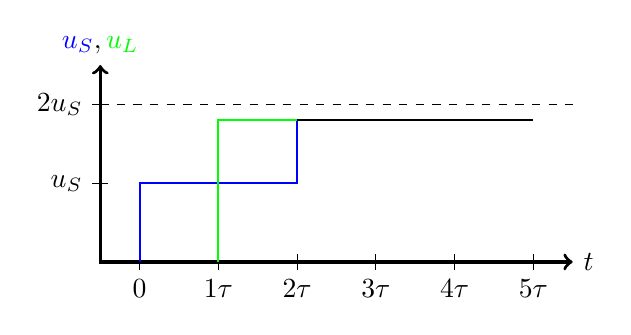
\begin{tikzpicture}
%	\HelpCords{0}{0}{7}{3}
	
	%Achsen
	\draw[very thick, <->]
	(0,2.5) node[above] {$\color{blue} u_S \color{black}, \color{green} u_L$} -- (0,0) -- (6,0)
	node[right] {$t$};
	
	%Beschriftung t-Achse
	\draw (0.5, 0.1) -- (0.5, -0.1) node[below]	{$0$};
	\draw (1.5, 0.1) -- (1.5, -0.1) node[below]	{$1\tau$};
	\draw (2.5, 0.1) -- (2.5, -0.1) node[below]	{$2\tau$};
	\draw (3.5, 0.1) -- (3.5, -0.1) node[below]	{$3\tau$};
	\draw (4.5, 0.1) -- (4.5, -0.1) node[below]	{$4\tau$};
	\draw (5.5, 0.1) -- (5.5, -0.1) node[below]	{$5\tau$};
	
	%Beschriftung u-Achse
	\draw (0.1, 1) -- (-0.1, 1) node[left]	{$u_S$};
	\draw (0.1, 2) -- (-0.1, 2) node[left]	{$2u_S$};
	\draw[dashed] (0,2) -- (6,2);
	
	%u_S
	\draw[thick, blue]
	(0.5, 0) --
	(0.5, 1) --
	(2.5, 1) --
	(2.5, 1.8) 
	;
	
	%u_L
	\draw[thick, green]
	(1.5, 0) --
	(1.5, 1.8) --
	(2.5, 1.8)
	;
	
	%u_S und u_L
	\draw[thick]
	(2.5, 1.8) -- 
	(5.5,1.8)
	;
		
\end{tikzpicture}
}
	\end{minipage}
	\begin{minipage}{0.39\textwidth}
		\begin{align*}
			\Gamma &= \frac{U_-}{U_+} = \frac{Z_L-Z_{ref}}{Z_L+Z_{ref}}\\
			&= \frac{1k\Omega-100\Omega}{1k\Omega+100\Omega}\\
			&= \frac{900\Omega}{1100\Omega} = 0.818
		\end{align*}
	\end{minipage}
\end{karte}

\begin{karte}{Wie sehen die Reflexionen bei folgender Anordnung aus?\\
		\scalebox{.8}{%Autor: Simon Walker
%Version: 1.0
%Datum: 09.06.2020
%Lizenz: CC BY-NC-SA

\begin{circuitikz}
	%\HelpCords{0}{0}{8}{3}
	
	
	\draw
	%Knoten
	(0, 0) coordinate (n1)
	(0, 3) coordinate (n2)
	(2, 3) coordinate (n3)
	(6, 3) coordinate (n4)
	(7, 3) coordinate (n5)
	(7, 0) coordinate (n6)	
	
	
	%Nur zu Hilfszwecken
%	(n1) node[above] {$n1$}
%	(n2) node[above] {$n2$}
%	(n3) node[above] {$n3$}
%	(n4) node[above] {$n4$}
%	(n5) node[above] {$n5$}
%	(n6) node[above] {$n6$}
	
	(n2) to[sV=${u_S}$] (n1) node[rground]{}
	(n2) to[R=${100\Omega}$] (n3)
	(n4) to[short] (n5) to[R, l_=${10\Omega}$, v^=${u_L}$] (n6) node[rground]{}
	;
	
	%Leitung
	\draw
	(n3) to[short] ($(n3)+(0.5, 0)$)
	(n4) to[short] ($(n4)+(-2, 0)$);
	
	\draw[fill=white] ($(n4)+(-0.5, 0)$) ellipse circle [x radius=0.3, y radius=0.5];
	\fill[white] ($(n3)+(0.5, -0.5)$) rectangle ($(n4)+(-0.5, 0.5)$);
	\draw ($(n3)+(0.5, 0)$) ellipse circle [x radius=0.3, y radius=0.5];
	\draw ($(n3)+(0.5, -0.5)$) -- ($(n4)+(-0.5, -0.5)$);
	\draw ($(n3)+(0.5, +0.5)$) -- ($(n4)+(-0.5, +0.5)$);
	
	
	\path ($(n3)+(0,+0.5)$) -- 
	node[above] {$100\Omega$}
	($(n4)+(0,+0.5)$);
	
	\draw[red,|->] ($(n3)-(0,0.8)$) -- 
	node[below, red] {$t=\tau$}
	($(n4)-(0,0.8)$);

\end{circuitikz}
}}
	Zum Zeitpunkt $t=0$ wird die Welle mit der Spannung $u_S$ losgeschickt. Zum Zeitpunkt $t=\tau$ kommt die Welle an der Last an. Da die Last zu niederohmig ist, wird eine Negative Welle mit $\Gamma u_S$ reflektiert. Nach $2\tau$ kommt die  beim Sender an und führt zu einer geringeren Spannung.\\
	\begin{minipage}{0.59\textwidth}
		\scalebox{.75}{%Autor: Simon Walker
%Version: 1.0
%Datum: 09.06.2020
%Lizenz: CC BY-NC-SA

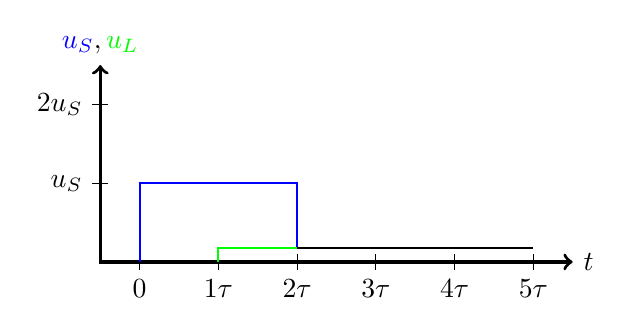
\begin{tikzpicture}
%	\HelpCords{0}{0}{7}{3}
	
	%Achsen
	\draw[very thick, <->]
	(0,2.5) node[above] {$\color{blue} u_S \color{black}, \color{green} u_L$} -- (0,0) -- (6,0)
	node[right] {$t$};
	
	%Beschriftung t-Achse
	\draw (0.5, 0.1) -- (0.5, -0.1) node[below]	{$0$};
	\draw (1.5, 0.1) -- (1.5, -0.1) node[below]	{$1\tau$};
	\draw (2.5, 0.1) -- (2.5, -0.1) node[below]	{$2\tau$};
	\draw (3.5, 0.1) -- (3.5, -0.1) node[below]	{$3\tau$};
	\draw (4.5, 0.1) -- (4.5, -0.1) node[below]	{$4\tau$};
	\draw (5.5, 0.1) -- (5.5, -0.1) node[below]	{$5\tau$};
	
	%Beschriftung u-Achse
	\draw (0.1, 1) -- (-0.1, 1) node[left]	{$u_S$};
	\draw (0.1, 2) -- (-0.1, 2) node[left]	{$2u_S$};
%	\draw[dashed] (0,2) -- (6,2);
	
	%u_S
	\draw[thick, blue]
	(0.5, 0) --
	(0.5, 1) --
	(2.5, 1) --
	(2.5, 0.18) 
	;
	
	%u_L
	\draw[thick, green]
	(1.5, 0) --
	(1.5, 0.18) --
	(2.5, 0.18)
	;
	
	%u_S und u_L
	\draw[thick]
	(2.5, 0.18) -- 
	(5.5,0.18)
	;
		
\end{tikzpicture}
}
	\end{minipage}
	\begin{minipage}{0.39\textwidth}
		\begin{align*}
		\Gamma &= \frac{U_-}{U_+} = \frac{Z_L-Z_{ref}}{Z_L+Z_{ref}}\\
		&= \frac{10\Omega-100\Omega}{10\Omega+100\Omega}\\
		&= \frac{-90\Omega}{110\Omega} = -0.818
		\end{align*}
	\end{minipage}
\end{karte}

\begin{karte}{Wie sehen die Reflexionen bei folgender Anordnung aus?\\
		\scalebox{.8}{%Autor: Simon Walker
%Version: 1.0
%Datum: 09.06.2020
%Lizenz: CC BY-NC-SA

\begin{circuitikz}
	%\HelpCords{0}{0}{8}{3}
	
	
	\draw
	%Knoten
	(0, 0) coordinate (n1)
	(0, 3) coordinate (n2)
	(2, 3) coordinate (n3)
	(6, 3) coordinate (n4)
	(7, 3) coordinate (n5)
	(7, 0) coordinate (n6)	
	
	
	%Nur zu Hilfszwecken
%	(n1) node[above] {$n1$}
%	(n2) node[above] {$n2$}
%	(n3) node[above] {$n3$}
%	(n4) node[above] {$n4$}
%	(n5) node[above] {$n5$}
%	(n6) node[above] {$n6$}
	
	(n2) to[sV=${u_S}$] (n1) node[rground]{}
	(n2) to[R=${10\Omega}$] (n3)
	(n4) to[short] (n5) to[R, l_=${100\Omega}$, v^=${u_L}$] (n6) node[rground]{}
	;
	
	%Leitung
	\draw
	(n3) to[short] ($(n3)+(0.5, 0)$)
	(n4) to[short] ($(n4)+(-2, 0)$);
	
	\draw[fill=white] ($(n4)+(-0.5, 0)$) ellipse circle [x radius=0.3, y radius=0.5];
	\fill[white] ($(n3)+(0.5, -0.5)$) rectangle ($(n4)+(-0.5, 0.5)$);
	\draw ($(n3)+(0.5, 0)$) ellipse circle [x radius=0.3, y radius=0.5];
	\draw ($(n3)+(0.5, -0.5)$) -- ($(n4)+(-0.5, -0.5)$);
	\draw ($(n3)+(0.5, +0.5)$) -- ($(n4)+(-0.5, +0.5)$);
	
	
	\path ($(n3)+(0,+0.5)$) -- 
	node[above] {$100\Omega$}
	($(n4)+(0,+0.5)$);
	
	\draw[red,|->] ($(n3)-(0,0.8)$) -- 
	node[below, red] {$t=\tau$}
	($(n4)-(0,0.8)$);

\end{circuitikz}}}
	Zum Zeitpunkt $t=0$ wird die Welle mit der Spannung $u_S$ losgeschickt. Allerdings wird diese sofort Reflektiert. Es kommt zu einer Spannungsüberhöhung an der Quelle ($Z_{ref}$ ist in diesem Fall $10\Omega$). Die Welle wird dann mit $u_S (1+\Gamma)$ losgeschickt und kommt dann zum Zeitpunkt $t=2\tau$ beim Empfänger an. Dort kommt es zu keiner Reflexion.\\
	\begin{minipage}{0.59\textwidth}
		\scalebox{.75}{%Autor: Simon Walker
%Version: 1.0
%Datum: 09.06.2020
%Lizenz: CC BY-NC-SA

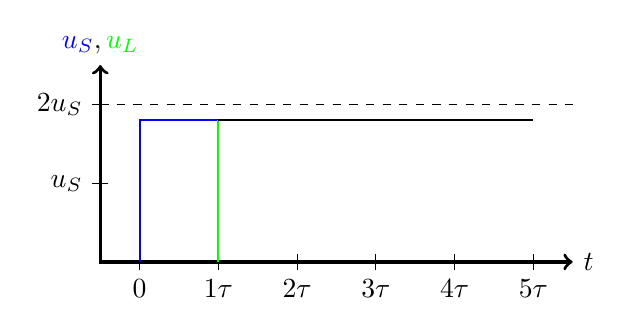
\begin{tikzpicture}
%	\HelpCords{0}{0}{7}{3}
	
	%Achsen
	\draw[very thick, <->]
	(0,2.5) node[above] {$\color{blue} u_S \color{black}, \color{green} u_L$} -- (0,0) -- (6,0)
	node[right] {$t$};
	
	%Beschriftung t-Achse
	\draw (0.5, 0.1) -- (0.5, -0.1) node[below]	{$0$};
	\draw (1.5, 0.1) -- (1.5, -0.1) node[below]	{$1\tau$};
	\draw (2.5, 0.1) -- (2.5, -0.1) node[below]	{$2\tau$};
	\draw (3.5, 0.1) -- (3.5, -0.1) node[below]	{$3\tau$};
	\draw (4.5, 0.1) -- (4.5, -0.1) node[below]	{$4\tau$};
	\draw (5.5, 0.1) -- (5.5, -0.1) node[below]	{$5\tau$};
	
	%Beschriftung u-Achse
	\draw (0.1, 1) -- (-0.1, 1) node[left]	{$u_S$};
	\draw (0.1, 2) -- (-0.1, 2) node[left]	{$2u_S$};
	\draw[dashed] (0,2) -- (6,2);
	
	%u_S
	\draw[thick, blue]
	(0.5, 0) --
	(0.5, 1.8) --
	(1.5, 1.8)
	;
	
	%u_L
	\draw[thick, green]
	(1.5, 0) --
	(1.5, 1.8)
	;
	
	%u_S und u_L
	\draw[thick]
	(1.5, 1.8) -- 
	(5.5,1.8)
	;
		
\end{tikzpicture}
}
	\end{minipage}
	\begin{minipage}{0.39\textwidth}
		\begin{align*}
		\Gamma &= \frac{U_-}{U_+} = \frac{Z_L-Z_{ref}}{Z_L+Z_{ref}}\\
		&= \frac{100\Omega-10\Omega}{100\Omega+10\Omega}\\
		&= \frac{90\Omega}{110\Omega} = 0.818
		\end{align*}
	\end{minipage}
\end{karte}

\begin{karte}{Bestimme die Reflexionen folgender Schaltung mit dem Bergeron-Verfahren!
		\scalebox{.6}{%Autor: Simon Walker
%Version: 1.0
%Datum: 15.06.2020
%Lizenz: CC BY-NC-SA

\begin{circuitikz}
	%\HelpCords{0}{0}{8}{3}
	
	
	\draw
	%Knoten
	(0, 0) coordinate (n1)
	(0, 3) coordinate (n2)
	(2, 3) coordinate (n3)
	(6, 3) coordinate (n4)
	(7, 3) coordinate (n5)
	(7, 0) coordinate (n6)
	
	
	%Nur zu Hilfszwecken
	%	(n1) node[above] {$n1$}
	%	(n2) node[above] {$n2$}
	%	(n3) node[above] {$n3$}
	%	(n4) node[above] {$n4$}
	%	(n5) node[above] {$n5$}
	%	(n6) node[above] {$n6$}
	;
	\draw[green]	
	(n2) to[esource=${u_S}$, color=green] (n1) node[rground]{}
	(n2) to[R=${Z_S}$, color=green] (n3);
	
	\draw[blue]
	(n4) to[short] (n5) to[R, l_=${Z_L}$, v^=${u_L}$, color=blue] (n6) node[rground]{};
	
	%Step generator symbol
	\path (n2) -- 
	node{\begin{tikzpicture}
		\draw[green] (-0.25,-0.15) -- (0,-0.15) -- (0, 0.15) -- (0.25, 0.15);
		\end{tikzpicture}}
	(n1); 
	
	%Leitung
	\draw[red]
	(n3) to[short] ($(n3)+(0.5, 0)$)
	(n4) to[short] ($(n4)+(-2, 0)$);
	
	\draw[red, fill=white] ($(n4)+(-0.5, 0)$) ellipse circle [x radius=0.3, y radius=0.5];
	\fill[white] ($(n3)+(0.5, -0.5)$) rectangle ($(n4)+(-0.5, 0.5)$);
	\draw[red] ($(n3)+(0.5, 0)$) ellipse circle [x radius=0.3, y radius=0.5];
	\draw[red] ($(n3)+(0.5, -0.5)$) -- ($(n4)+(-0.5, -0.5)$);
	\draw[red] ($(n3)+(0.5, +0.5)$) -- ($(n4)+(-0.5, +0.5)$);
	
	
	\path ($(n3)+(0,+0.5)$) -- 
	node[above, red] {$Z_0$}
	($(n4)+(0,+0.5)$);
	
	\draw[red,|->] ($(n3)-(0,0.8)$) -- 
	node[below, red] {$t=\tau$}
	($(n4)-(0,0.8)$);
	
\end{circuitikz}
}\\
		 \small $\color{green}Z_S = 25\Omega$, $\color{red}Z_0 = 50\Omega$, $\color{blue}Z_L = 100\Omega$}
	\scalebox{.82}{%Autor: Simon Walker
%Version: 1.0
%Datum: 09.06.2020
%Lizenz: CC BY-NC-SA

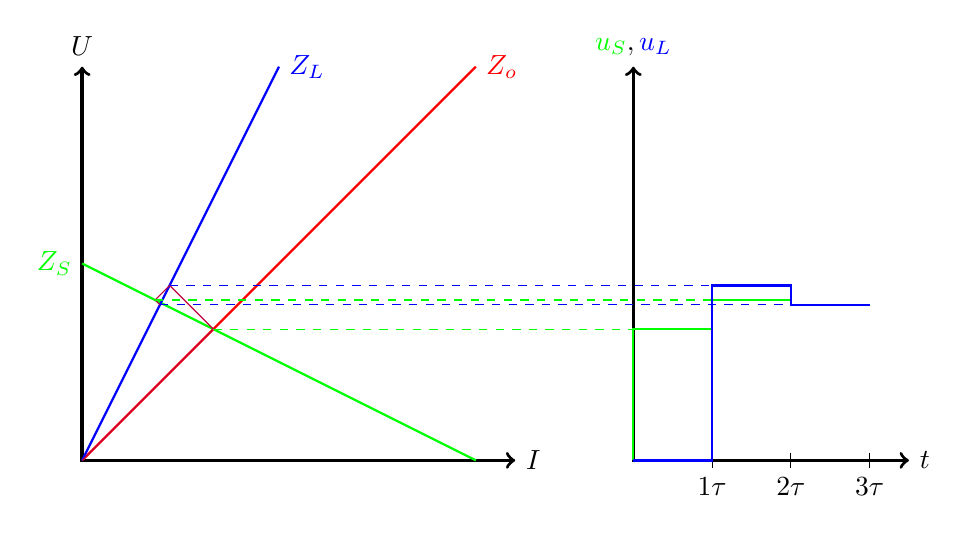
\begin{tikzpicture}
	%\HelpCords{0}{0}{12}{6}
	%Achsen
	\draw[very thick, <->]
	(0,5) node[above] {$U$} -- (0,0) -- (5.5,0)
	node[right] {$I$};
	
	\draw[very thick, <->]
	(7,5) node[above] {$\color{green} u_S \color{black}, \color{blue} u_L$} -- (7,0) -- (10.5,0)
	node[right] {$t$};
	
	%Beschriftung t-Achse
	\draw (8, 0.1) -- (8, -0.1) node[below]	{$1\tau$};
	\draw (9, 0.1) -- (9, -0.1) node[below]	{$2\tau$};
	\draw (10, 0.1) -- (10, -0.1) node[below] {$3\tau$};

	
	%Z_S
	\draw[thick, green] (0, 2.5) node[left, green] {$Z_S$} -- (5, 0); %yS=-0.5x+2.5
	
	%Z_0
	\draw[thick, red] (0, 0) -- (5, 5) node[right, red] {$Z_o$}; %y0=x
	
	%Z_L
	\draw[thick, blue] (0, 0) -- (2.5, 5) node[right, blue] {$Z_L$}; %yL=2x
	
	%Welle
	%Berechnungen
	%SP1: yS=y0 (1.6666, 1.6666) 
	%SP1-SP2 y1=-x+3.3333
	%SP2: yL=y1 (1.1111, 2.2222)
	%SP2--SP3 y2=x+1.1111
	%SP3: yS=y2 (0.9259, 2.0370)
	%SP3--SP4 y3=-x+2.9629
	%SP4: yL=y3 (0.9876, 1.9752)
	
	\draw[purple] (0,0) -- (1.6666, 1.6666) -- (1.1111, 2.2222) -- (0.9259, 2.0370) -- (0.9876, 1.9752);
	
	%t=0
	\draw[dashed, green] (1.6666, 1.6666) -- (7, 1.6666);
	
	%t=1tau
	\draw[dashed, blue] (1.1111, 2.2222) -- (8, 2.2222);
	
	%t=2tau
	\draw[dashed, green] (0.9259, 2.0370) -- (9, 2.0370);
	
	%t=3tau
	\draw[dashed, blue] (0.9876, 1.9752) -- (10, 1.9752);
	
	%u_S
	\draw[thick, green] (7, 0) -- (7, 1.6666) -- (8, 1.6666) -- (8, 2.0370) -- (9, 2.0370);
	\draw[thick, blue] (7, 0) --(8, 0) -- (8, 2.2222) -- (9, 2.2222) -- (9, 1.9752) -- (10, 1.9752);
	
	
		
\end{tikzpicture}
}
	 
\end{karte}

\begin{karte}{Was ist eine Leitungstransformation?}
	\scalebox{.6}{%Autor: Simon Walker
%Version: 1.0
%Datum: 17.06.2020
%Lizenz: CC BY-NC-SA

\begin{circuitikz}
	%\HelpCords{0}{0}{8}{3}
	
	
	\draw
	%Knoten
%	(0, 0) coordinate (n1)
	(0, 3) coordinate (n2)
	(1, 3) coordinate (n3)
	(5, 3) coordinate (n4)
	(6, 3) coordinate (n5)
	(6, 0) coordinate (n6)	
	
	
	%Nur zu Hilfszwecken
%	(n1) node[above] {$n1$}
%	(n2) node[above] {$n2$}
%	(n3) node[above] {$n3$}
%	(n4) node[above] {$n4$}
%	(n5) node[above] {$n5$}
%	(n6) node[above] {$n6$}
	
	(n2) to[short,o-] (n3)
	(n4) to[short] (n5) to[R=${Z_a}$] (n6) node[rground]{}
	;
	
	%Leitung
	\draw
	(n3) to[short] ($(n3)+(0.5, 0)$)
	(n4) to[short] ($(n4)+(-2, 0)$);
	
	\draw[fill=white] ($(n4)+(-0.5, 0)$) ellipse circle [x radius=0.3, y radius=0.5];
	\fill[white] ($(n3)+(0.5, -0.5)$) rectangle ($(n4)+(-0.5, 0.5)$);
	\draw ($(n3)+(0.5, 0)$) ellipse circle [x radius=0.3, y radius=0.5];
	\draw ($(n3)+(0.5, -0.5)$) -- ($(n4)+(-0.5, -0.5)$);
	\draw ($(n3)+(0.5, +0.5)$) -- ($(n4)+(-0.5, +0.5)$);
	
	
	
	\path ($(n3)+(0,0.5)$) -- 
	node[above] {$Z_0$}
	($(n4)+(0,0.5)$);
	
	
	\draw[<-, very thick] ($(n2)+(0,-1)$) -| ++(-0.8,-0.5) node[below] {$Z?$};
	
	\draw[blue,|<->|] ($(n3)-(0,0.8)$) -- 
	node[below, blue] {$l/\lambda$}
	($(n4)-(0,0.8)$);
	

\end{circuitikz}
}\\
	Um Herauszufinden welche Impedanz die Quelle sieht, muss eine Leitungstransformation durchgeführt werden. Die Impedanz ist stark von der Länge der Leitung abhängig.
	Bei einer Leitungslänge von $l=\lambda/4$ gilt folgende vereinfachte Formel:
	\fbox{$Z_{\lambda/4} \cdot Z_A = {Z_0}^2$}
\end{karte}

\begin{karte}{Was zeigt ein Smith-Chart?}
	\begin{compactitem}
		\item Aufzeichnen des Komplexen Reflexionsfaktor in der Komplexen ebene von $\Gamma$
		\item Eine Ortskurve des Komplexen Reflexionszeigers
		\item Die Bilinear Transformation der Normierten Impedanz
	\end{compactitem}
	\centering
	\scalebox{.4}{%Autor: Simon Walker
%Version: 1.0
%Datum: 17.06.2020
%Lizenz: CC BY-NC-SA

\usepgfplotslibrary{smithchart}

\begin{tikzpicture}

\begin{smithchart}[width=10cm,
	smithchart mirrored,
	yticklabel around circle,
	xticklabel shift=-19pt,
	]
	
\end{smithchart}
\begin{smithchart}[width=10cm,
	grid style={black},
	yticklabel around circle*,
	]
	
	
\end{smithchart}

\end{tikzpicture}
}
\end{karte}

\begin{karte}{Was für eine Impedanz und Admittanz zeigt folgendes $50\Omega$ Smith-Chart?
		\scalebox{.4}{%Autor: Simon Walker
%Version: 1.0
%Datum: 25.06.2020
%Lizenz: CC BY-NC-SA


\begin{tikzpicture}

\begin{smithchart}[width=10cm,
	smithchart mirrored,
	yticklabel around circle,
	xticklabel shift=-19pt]
\end{smithchart}

\begin{smithchart}[width=10cm,
	grid style={black},
	yticklabel around circle*]
	\draw[red,fill=red] (0.5,0.5) circle (0.2cm);
\end{smithchart}

\end{tikzpicture}
}}
	\centering
	\scalebox{.35}{%Autor: Simon Walker
%Version: 1.0
%Datum: 25.06.2020
%Lizenz: CC BY-NC-SA


\begin{tikzpicture}

\begin{smithchart}[width=10cm,
	smithchart mirrored,
	yticklabel around circle,
	xticklabel shift=-19pt]
	\draw[green, thick, domain=-20:20,smooth,variable=\x, samples=100] plot (1,\x);
	\draw[green, thick, domain=0:20,smooth,variable=\x, samples=100] plot (\x,1);
\end{smithchart}

\begin{smithchart}[width=10cm,
	grid style={black},
	yticklabel around circle*]
	\draw[blue, thick, domain=-10:10,smooth,variable=\x, samples=100] plot (0.5,\x);
	\draw[blue, thick, domain=0:20,smooth,variable=\x, samples=100] plot (\x,0.5);
	\draw[red,fill=red] (0.5,0.5) circle (0.2cm);
\end{smithchart}

\end{tikzpicture}
}
	\flushleft \vspace{-12pt}
	Aus dem Diagramm lässt sich die Impedanz und die Admittanz sehr einfach auslesen. Dazu muss den Kreisen gefolgt werden. Für die Impedanz (Blau):\\
	$Z = Z_0 \cdot (0.5 + j0.5) = 50\Omega \cdot (0.5 + j0.5) = (25 + j25)\Omega$\\
	Für die Admittanz (Grün) sind die Werte oben Negativ:\\
	$Y = Y_0 \cdot (1 - j1) = \frac{1}{50\Omega} \cdot (1 - j1) = (20 - j20)mS$
\end{karte}

\begin{karte}{Ab wann muss eine Leitung als solches betrachtet werden?}
	Entscheidend  ist die Länge der Leitung im Bezug zur Wellenlänge. Ist die Leitung viel kürzer als die Wellenlänge $l<<\lambda$ (bsp $l \approx \frac{\lambda}{100}$) haben wir keine Probleme und müssen die Leitung nicht als solches betrachten. Bei höheren Frequenzen oder längeren Leitungen wird es langsam kritisch $\color{red} l \approx \frac{\lambda}{20} \dots \frac{\lambda}{10}$. Dann muss die Leitung auch als Leitung betrachten werden. Die Grenze variiert stark mit den Qualitätsanforderungen der Schaltung.
\end{karte}

\begin{karte}{Weshalb ist der Einsatz von Koaxialkabeln elektrisch begrenzt?}
	Koaxialkabel können wir ab DC bis in den GHz-Bereich benützen. Der Grund dafür ist, dass ab einer gewissen Frequenz der mittlere Umfang $U$ des Koaxialkabels nicht mehr sehr klein ist gegenüber $\lambda$.
	Dann beginnt sich der Sogenannte 2. Mode auszubreiten. Die Überlagerungen der beiden Modes kann zu beliebigen Auslöschung und Verzerrungsefekte führen.
	
	\centering{\scalebox{.7}{%Autor: Simon Walker
%Version: 1.0
%Datum: 25.06.2020
%Lizenz: CC BY-NC-SA


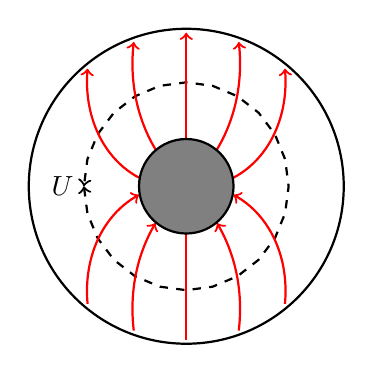
\begin{tikzpicture}

%Mittlerer Umfang
\draw[<->, 
dashed, 
thick, 
domain=180:540, 
variable=\x] 
plot ({1.3*cos(\x)}, {1.32*sin(\x)})
node[left] {$U$};


%Feldlinien
\draw[red, thick, ->] (0, 0.6) -- (0, 1.95);
\draw[red, thick, ->, domain=0.61:1.95, variable=\x] plot ({130-20/(1.35/(\x-0.6))}:\x);
\draw[red, thick, ->, domain=0.61:1.95, variable=\x] plot ({50+20/(1.35/(\x-0.6))}:\x);
\draw[red, thick, ->, domain=0.61:1.95, variable=\x] plot ({170-40/(1.35/(\x-0.6))}:\x);
\draw[red, thick, ->, domain=0.61:1.95, variable=\x] plot ({10+40/(1.35/(\x-0.6))}:\x);

\draw[red, thick, <-] (0, 0.6) -- (0, -1.95);
\draw[red, thick, <-, domain=0.61:1.95, variable=\x] plot ({-130+20/(1.35/(\x-0.6))}:\x);
\draw[red, thick, <-, domain=0.61:1.95, variable=\x] plot ({-50-20/(1.35/(\x-0.6))}:\x);
\draw[red, thick, <-, domain=0.61:1.95, variable=\x] plot ({-170+40/(1.35/(\x-0.6))}:\x);
\draw[red, thick, <-, domain=0.61:1.95, variable=\x] plot ({-10-40/(1.35/(\x-0.6))}:\x);


\draw[thick] (0,0) circle (2); %Ausserer Kreis
\draw[thick, fill=gray] circle (0.6); %Innerer Kreis
\end{tikzpicture}
}}
			
\end{karte}
